\chapter{Conclusion}
\label{ch:conclusion}

\begin{figure}[h]
\centering
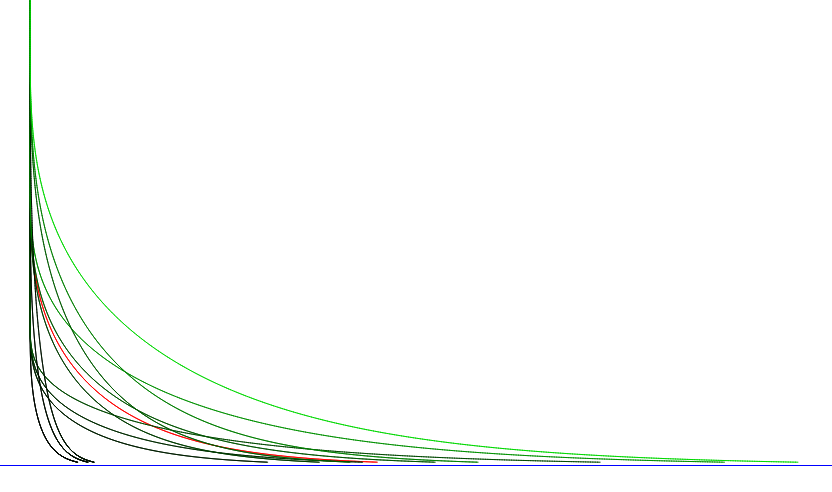
\includegraphics[width=0.7\textwidth]{fun_different_hybrid_path_curves}
\caption{Artwork of different path drawn via Hybrid formulation}
\end{figure}

This thesis successfully demonstrated that unified guidance considering both Multirotor and Fixed Wing use cases for a Hybrid VTOL can be formulated. The Hybrid formulation\ref{eq:hybrid_velocity_components}, was designed to satisfy all the constraints\ref{ch:problem_definition} and hence is a better solution for the use in Hybrid VTOLs.\\

Furthermore, more analysis was given in \autoref{sec:evaluation}, where the superiority of the Hybrid formulation over original Unicyclic method was shown. This is in most part, thanks to the adjustability of the $t_{const}$ appropriately by predicting the acceleration that will occur when following a path beforehand.\\

Note, however that in order to utilize this fully, the real-time adaptation of the $t_{const}$ should be done carefully, to not violate acceleration constraints of different modes of operation.

\section{Future Work}

\subsection{Real Flight Testing}
Unfortunately, the proposed methods were never tested on a real test flight. Implementation of this algorithm on open-source flight control software such as PX4 Autopilot\cite{noauthor_px4_2023} would certainly be possible in the future.

\subsection{Acceleration Limit in Body Frame}
One of the biggest reason why the Maximum Acceleration Method

\subsection{Wind}
Since the acceleration constraint of a Fixed Wing is tied to it's yaw angle, which in turn is tied to the wind vector, it wasn't trivial to come up with a generic solution that would cover all the different wind cases in terms of the acceleration required by the Vector Field.

Therefore, it would be nice to incorporate wind more thoroughly in the guidance algorithm in the future for both Multirotor and Fixed Wing cases to create an actually optimal path following commands, and not just the ground velocity vector field.

\subsection{Low Level Control}
This thesis assumed that the low level controller would be capable of actuating the vehicle to track it's desired ground velocity. However, without the acceleration feed forward command directly computed from the spatial derivative of the Vector Field it would of course be challenging for the low level controller to tightly track the desired velocity.

Therefore, like done in the original unicyclic formulation, it is desirable to passthrough an actual acceleration command in body frame.